\section{Rayonnement dipolaire électrique}

Le rayonnement électromagnétique est un phénomène fondamental. Toute charge en mouvement accéléré rayonne un champ [$\vec{E},\vec{B}$] et donc de l'énergie électromagnétique.

\subsection{Le modèle du dipôle électrique oscillant}

On a une distribution neutre, et on fait l'hypothèse que les charges mobiles sont en mouvement sinusoïdal. Par exemple, un atome possède une charge $q>0$ fixe (le noyau) et une charge $-q<0$ mobile (électrons). On peut donc le modéliser avec un dipôle comme à la Figure~\ref{fig:modelisation_atome_dipole_oscillant}. Dans ce cas, le mouvement est~$z(t)=z_{0}\cos(\omega t)$ où $z_{0}$ est la distance typique entre le noyau et l'électron, et le moment dipolaire est donc
\begin{equation*}
    \boxed{
        \vec{p}(t)=q\vec{G^{-}O}(t)=-qz_{0}\cos(\omega t)\vec{u_{z}}.
    }
\end{equation*}

\begin{figure}
    \centering
    \tikzsetnextfilename{modelisation_atome_dipole_oscillant}
    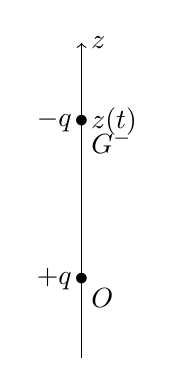
\begin{tikzpicture}[scale=1]  
        % \helpgrid{3}{3}
        \draw[->] (0,0)--++(0,4) node [right] {$z$};
        \node at (0,3) {$\bullet$};
        \node at (0,3) [left] {$-q$};
        \node at (0,3) [right] {$z(t)$};
        \node at (0,3) [below right] {$G^{-}$};
        \node at (0,1) {$\bullet$};
        \node at (0,1) [left] {$+q$};
        \node at (0,1) [below right] {$O$};
    \end{tikzpicture}
    \caption{Modélisation d'un atome par un dipôle électrique oscillant.}    
    \label{fig:modelisation_atome_dipole_oscillant}
\end{figure}

En ordre de grandeur, on a $p_{0}\sim 10^{-29}\si{\coulomb\metre}$ (environ 1 Debye), et $\omega\sim 10^{15}\si{\radian\per\second}$. Pour une antenne, on a $f\sim 100\si{\mega\hertz}$ d'où $\lambda\sim 3\si{\metre}$. Ainsi, la longueur d'une antenne est typiquement de l'ordre de la longueur d'onde.

\subsection{Les trois échelles de longueur}

On a accès à trois longueurs : $z_{0}$ qui est la longueur typique entre la charge positive et la charge négative, $\lambda=c/f$ qui est la longueur d'onde de l'onde sinusoïdale, et $r$ qui est la distance de l'observateur au dipôle.

Plusieurs hypothèses permettent de distinguer ces trois longueurs:
\begin{itemize}
    \item \textbf{Approximation dipolaire} : $z_{0}\ll r$;
    \item \textbf{Mouvement des charges non relativiste} : la vitesse maximale entre les deux charges doit être bien plus petite que la vitesse de la lumière, d'où $\omega z_{0}\ll c$, ce qui revient, comme $c/\omega = \lambda/(2\pi)$, à $z_{0}\ll\lambda$.
    \item \textbf{Champ lointain ou zone de rayonnement} : on suppose le phénomène de propagation prépondérant, et donc le temps de propagation est très grand devant la période du dipôle, d'où $r/c\gg T$ (c'est l'inverse de l'ARQS), d'où $r\gg cT=\lambda$.
\end{itemize}

Ainsi, on a
\begin{equation*}
    \boxed{
        z_{0}\ll \lambda\ll r.
    }
\end{equation*}

\subsection{Champ électromagnétique dans la zone de rayonnement : approche qualitative}

\subsubsection{Symétries}

On se place en coordonnées sphériques $(r,\theta,\varphi)$, le dipôle étant en O et orienté selon l'axe $\vec{u_z}$:
\begin{itemize}
    \item symétrie de révolution par rapport à l'axe (Oz) : pas de dépendance en~$\varphi$;
    \item tout plan qui contient (Oz) est un plan de symétrie : le champ magnétique est selon~$\vec{u_{\varphi}}$ et le champ électrique est nul selon cette même direction.
\end{itemize}

Finalement,
\begin{equation*}
    \boxed{
        \vec{B}=B(r,\theta,t)\vec{u_{\varphi}},\qquad
        \vec{E}=E_{r}(r,\theta,t)\vec{u_r}+E_{\theta}(r,\theta,t)\vec{u_{\theta}}.
    }
\end{equation*}

\subsubsection{Charges accélérées}

L'électromagnétisme étant une théorie linéaire, l'intensité des champs magnétique et électrique sont proportionnels à l'accélération des charges :
\begin{equation*}
    \boxed{
        E,B\propto q\ddot{z}\propto\ddot{p}.
    }
\end{equation*}

\subsubsection{Temps de propagation}

La propagation de l'onde est radiale et à vitesse finie~$c$. Ainsi, le temps de propagation est~$\tau_{\rm propa}=r/c$. Le champ électromagnétique en un point $M$ à l'instant $t$ généré par le dipôle~$\vec{p}$ est donc lié aux valeurs de~$\vec{p}$ à l'instant $t-\tau_{\rm propa}=t-r/c$. Ainsi,
\begin{equation*}
    \boxed{
        \vec{B}(M,t)\propto\ddot{p}(t-r/c)\vec{u_{\varphi}},
    }
\end{equation*}
et de même pour le champ électrique.

\subsubsection{Conservation de l'énergie}

Comme on suppose une propagation dans le vide, la moyenne de la puissance rayonnée reste constante sur une sphère $S$ centrée autour du dipôle. Dans ce cas, on a 
\begin{equation*}
    \left\langle P_{\rm ray}\right\rangle=\oiint_{S}\left\langle\vec{\Pi}\right\rangle\cdot\vec{u_r}dS\approx\left\lVert\left\langle\vec{\Pi}\right\rangle\right\rVert_{\infty}4\pi r^{2}\approx{\rm constante}.
\end{equation*}
Donc~$\left\lVert\left\langle\vec{\Pi}\right\rangle\right\rVert_{\infty}\propto r^{-2}$. Or~$\Pi\sim E^{2},B^{2}$. Donc le champ électromagnétique décroît en~$1/r$. Finalement,
\begin{equation*}
    \boxed{
        \vec{B}(M,t)\propto\frac{1}{r}\ddot{p}(t-r/c)\vec{u_{\varphi}},
    }
\end{equation*}
et de même pour le champ électrique.

\subsubsection{Anisotropie du champ rayonné}

Si on se place sur l'axe du dipôle ($\theta=0,\pi$), alors le champ magnétique est nul et le champ électrique aussi. Donc~$\vec{\Pi}=\vec{0}$ sur l'axe : il n'y a aucune puissance rayonnée selon l'axe.

Si on se place dans le plan perpendiculaire à l'axe du dipôle ($\theta=\pi/2$), a priori les champs sont non nuls. On fait alors la conjecture que le champ électromagnétique est maximal dans ce plan. Le plus simple pour satisfaire cette conjecture et l'observation précédente est que~$E,B\propto\sin\theta$.
Finalement,
\begin{equation*}
    \boxed{
        \vec{B}(M,t)\propto\frac{\sin\theta}{r}\ddot{p}(t-r/c)\vec{u_{\varphi}},
    }
\end{equation*}
et de même pour le champ électrique.

\subsubsection{Structure locale d'OPP dans la ZR}

Dans la zone de rayonnement, on a~$r\gg\lambda$. La propagation est radiale, les surfaces d'onde sont strictement des sphères de centre le dipôle. Étant très loin du dipôle, les sphères sont quasiment des plans tangents. L'onde rayonnée est donc quasiment plane, et comme l'OPP est selon~$\vec{u_r}$ (on est dans le vide), et que~$\vec{E}=c\vec{B}\wedge\vec{u_r}$, on a~$\vec{E}\propto cB\vec{u_{\theta}}$. Ainsi, dans la zone de rayonnement, on a
\begin{equation*}
    \boxed{
        \vec{E}(M,t)\propto\frac{c\sin\theta}{r}\ddot{p}(t-r/c)\vec{u_{\theta}},
    }
\end{equation*}
car~$\left\vert E_r\right\rvert\ll\left\lvert E_{\theta}\right\rvert$ dans ce cas.

\subsubsection{Analyse dimensionnelle}

Pour obtenir les ingrédients restants, soit~$k$ tel que~$\vec{B}=k\sin\theta\ddot{p}(t-z/c)\vec{u_{\varphi}}/r$. On sait que~$[B]=[\mu_0][i]/[L]=[\mu_0]\si{\coulomb\per\second\per\metre}$ via la formule du champ magnétique sur un solénoïde (par exemple). D'après ce qu'on a écrit, on a~$[B]=[k][\ddot{p}]/[r]=[k]\si{\coulomb\metre\per\second\squared}/\si{\metre}$. Finalement,~$[k]=[\mu_0]\si{\second\per\metre}=[\mu_0]/(\si{\metre\per\second})$. On conjecture donc que~$[k]={\rm constante}\mu_0/c$. Il se trouve que c'est la bonne chose et que la constante est simplement~$1/(4\pi)$. On obtient donc l'expression du champ électromagnétique dans la zone de rayonnement :
\begin{equation*}
    \boxed{
        \vec{B}=\frac{\mu_0}{4\pi c}\frac{\sin\theta}{r}\ddot{p}\left(t-\frac{r}{c}\right)\vec{u_{\varphi}},\qquad
        \vec{E}=\frac{\mu_0}{4\pi}\frac{\sin\theta}{r}\ddot{p}\left(t-\frac{r}{c}\right)\vec{u_{\theta}}.
    }
\end{equation*}

\subsection{Le champ rayonné : raisonnement en ordres de grandeur}

Dans l'approximation dipolaire, on a~$r\gg z_0$. Dans l'hypothèse non relativiste, on a~$\lambda\gg z_{0}$. Mais~$\lambda/r$ est quelconque. Il se trouve que la champ électromagnétique est donné par
\begin{equation*}
    \begin{aligned}
        \vec{E}&=\frac{\mu_0}{4\pi r}\begin{pmatrix}
            2\cos\theta\left(
                \frac{c^{2}}{r^{2}}p\left(t-\frac{r}{c}\right)+\frac{c}{r}\dot{p}\left(t-\frac{r}{c}\right)
            \right)\\
            \sin\theta\left(
                \frac{c^{2}}{r^{2}}p\left(t-\frac{r}{c}\right)+\frac{c}{r}\dot{p}\left(t-\frac{r}{c}\right)+\ddot{p}\left(t-\frac{r}{c}\right)
            \right)\\
            0
        \end{pmatrix},\\
        \vec{B}&=\frac{\mu_0}{4\pi c}\frac{\sin\theta}{r}\left(
            \frac{c}{r}\dot{p}\left(t-\frac{r}{c}\right)+\ddot{p}\left(t-\frac{r}{c}\right)
        \right)\vec{u_{\varphi}}.
    \end{aligned}
\end{equation*}

Regardons si on peut négliger certains termes. Dans la zone de rayonnement, on a~$r\gg\lambda$. Or,
\begin{equation*}
    \frac{\left\lvert\ddot{p}\right\rvert}{\left\lvert\frac{c}{r}\dot{p}\right\rvert}\sim\frac{\omega^{2}p_0}{\frac{c}{r}\omega p_0}=\frac{r\omega}{c}=\frac{2\pi r}{\lambda}\gg1.
\end{equation*}
De plus,
\begin{equation*}
    \frac{
        \left\lvert\frac{c}{r}\dot{p}\right\rvert
    }{
        \left\lvert\frac{c^{2}}{r^{2}}p\right\rvert
    }\sim\frac{\omega r}{c}\gg1.
\end{equation*}
Ainsi, on a~$\ddot{p}\gg\frac{c}{r}\dot{p}\gg\frac{c^{2}}{r^{2}}p$. Dans la zone de rayonnement, on a donc bien~$\left\lvert E_r\right\rvert\ll\left\lvert E_{\theta}\right\rvert$, et on retrouve bien l'expression précédente pour le champ électromagnétique.

\begin{remark}
    Dans la zone de champ proche (ARQS), on a~$\tau_{\rm propa}\ll T$, \emph{i.e.}~$r\ll\lambda$. Donc~$\ddot{p}\ll\frac{c}{r}\dot{p}\ll\frac{c^{2}}{r^{2}}p$. En négligeant le temps de propagation, \emph{i.e.}~$t-r/c\approx t$, on obtient
    \begin{equation*}
        \vec{E}=\frac{\mu_0}{4\pi r}\begin{pmatrix}
            2\cos\theta\frac{c^{2}}{r^{2}}p(t)\\
            \sin\theta\frac{c^{2}}{r^{2}}p(t)\\
            0
        \end{pmatrix}=\frac{p(t)}{4\pi\varepsilon_0 r^{3}}\begin{pmatrix}
            2\cos\theta\\\sin\theta\\0
        \end{pmatrix},
    \end{equation*}
    et
    \begin{equation*}
        \vec{B}=\frac{\mu_0}{4\pi c}\frac{\sin\theta}{r}\frac{c}{r}\dot{p}(t)\vec{u_{\varphi}}.
    \end{equation*}
    C'est la même expression qu'en statique.
\end{remark}

On peut se demander si, dans la zone de rayonnement, on peut négliger le champ magnétique par rapport au champ électrique. On a 
\begin{equation*}
    \frac{\left\lvert E\right\rvert}{c\left\lvert B\right\rvert}=
    \frac{
        \frac{p}{4\pi\varepsilon_0 r^{3}}
    }{
        c\frac{\mu_0\dot{p}}{4\pi r^{2}}
    }=\frac{r^{2}}{\mu_0\varepsilon_0 c\omega r^{3}}=\frac{c}{r\omega}=\frac{\lambda}{2\pi r}\gg 1.
\end{equation*}
C'est un bon début, mais il est encore plus pertinent de mesurer l'apport de chaque champ à l'énergie électromagnétique. On a alors
\begin{equation*}
    \frac{
        \frac{\varepsilon_0 E^{2}}{2}
    }{
        \frac{B^{2}}{2\mu_0}
    }=\mu_0\varepsilon_0\frac{c^{4}}{r^{2}\omega^{2}}=\frac{c^{2}}{r^{2}\omega^{2}}\gg1.
\end{equation*}
On peut donc considérer que l'on est dans l'ARQS électrique.

\subsection{Bilan : propriétés essentielles du champ électromagnétique rayonné dans la ZR}

\subsubsection{Structure locale de l'OPP}

Dans une zone de dimension~$\sim\lambda$ ($\ll r$), on a~$\frac{\sin\theta}{r}\approx{\rm constante}$ et~$(\vec{u_r},\vec{u_{\theta}},\vec{u_{\varphi}})\approx{\rm constante}$. Ainsi,~$\vec{E}(M,t)\approx\vec{E}(X,t)={\rm cte}\ddot{p}\left(t-\frac{X}{c}\right)\vec{u_{Y}}$ est transverse électrique (vrai que dans la ZR car~$\left\lvert E_r\right\rvert\ll\left\lvert E_{\theta}\right\rvert$), et ~$\vec{B}(M,t)=\vec{u_X}\wedge\frac{\vec{E}}{c}$. Localement, on a donc une OPP.

\subsubsection{Anisotropie du rayonnement}

Les champs sont proportionnels à~$\sin\theta$ : pas d'ondes rayonnées dans l'axe du dipôle, et rayonnement maximale à~$\theta=\pi/2$.

\subsubsection{Décroissance en 1/r}

Cette décroissance traduit la conservation de l'énergie. La décroissance en $1/r$ permet les télécommunications. En effet, supposons que le champ décroisse en~$r^{-1-\varepsilon}$ avec $0<\varepsilon\ll1$. Alors~$\vec{\Pi}\propto r^{-2(1+\varepsilon)}$ et donc~$\left\langle P\right\rangle\sim r^{-2\varepsilon}\xrightarrow[r\to+\infty]{}0$.

\subsubsection{Polarisation rectiligne}

On a~$\vec{E}(M,t)\parallel\vec{u_{\theta}}$, donc l'onde est polarisée selon~$\vec{u_{\theta}}$. Un cas particulier important est la polarisation dans le plan~$\theta=\pi/2$ : dans ce cas, le champ électrique est parallèle au dipôle, c'est-à-dire~$\vec{E}\parallel\vec{p}$.

\subsection{Vecteur de Poynting de la zone de rayonnement}

\subsubsection{Valeur instantanée et moyenne}

On a~$\vec{\Pi}(M,t)=\frac{E^{2}(M,t)}{\mu_0 c}\vec{u_r}$ d'où
\begin{equation*}
    \boxed{
        \vec{\Pi}(M,t)=
        \frac{\mu_0}{(4\pi)^{2}c}\left(\frac{\sin\theta}{r}\right)^{2}\left(
            \ddot{p}\left(t-\frac{r}{c}\right)
        \right)^{2}\vec{u_r}.
    }
\end{equation*}
Ainsi,~$\vec{\Pi}\parallel+\vec{u_r}$ : la propagation de l'énergie est selon~$+\vec{u_r}$. Localement, le vecteur de Poynting est une fonction de~$t-r/c$, la propagation est à vitesse $c$. Enfin, on a~$\left\lVert\vec{\Pi}\right\rVert\propto r^{-2}$.

Pour un mouvement sinusoïdal du dipôle~$p(t)=p_0\cos(\omega t)$, on obtient
\begin{equation*}
    \boxed{
        \left\langle\vec{\Pi}\right\rangle=\frac{\mu_0}{\pi^{2}c}\left(\frac{\sin\theta}{r}\right)^{2}p_0^{2}\omega^{4}\vec{u_r}\propto\omega^{4}.
    }
\end{equation*}

\subsubsection{Indicatrice de rayonnement}

Il s'agit de la directivité de l'émission. Le vecteur de Poynting est une fonction de~$\theta$, à rayon~$r$ fixé, et qui varie selon~$\sin^{2}\theta$. On se réfère à la Figure~\ref{fig:vecteur_Poynting_indicatrice_rayonnement}.

\begin{figure}
    \centering
    \tikzsetnextfilename{vecteur_Poynting_indicatrice_rayonnement}
    \begin{tikzpicture}[scale=1]  
        % \helpgrid{3}{3}
        \draw[->] (0,0)--++(0,3) node [above] {$z$};
        \draw[->] (-4,0)--++(8,0) node [right] {$x$};
        \draw[->, blue,text=blue, line width=0.5mm] (0,0)--++(0,2) node [left] {$\vec{p}$};
        \node[text=red] at (-3,0) {$\bullet$};
        \node[text=red] at (3,0) {$\bullet$};
        \node at (0,0) {$\bullet$};
        \draw[red] (0,0) to[out=45, in=135] (3,0);
        \draw[red] (0,0) to[out=-45, in=-135] (3,0);
        \draw[red] (-3,0) to[out=45, in=135] (0,0);
        \draw[red] (-3,0) to[out=-45, in=-135] (0,0);

        \draw[<-,text=red,draw=red] (3.1,-0.1)--(3.5,-0.5) node [right] {$\theta=\pi/2$};
        \draw[<-,text=red,draw=red] (-3.1,-0.1)--(-3.5,-0.5) node [left] {$\theta=3\pi/2$};
        \draw[<-,text=red,draw=red] (0,-0.1) to[out=-90,in=180] (1.5,-1) node [right] {$\theta\in\left\lbrace0,\pi\right\rbrace$};

        \draw[blue,->,text=blue] (0,0)--(2,0.55) node [above right] {$\left\lVert\left\langle\vec{\Pi}\right\rangle\right\rVert$};
        \centerarc[blue,text=blue](0,0)(90:15.5:1);
        \node[text=blue] at (0.9,0.9) {$\theta$};

        \draw[green, line width=0.4mm] (-1.25,-2)--(1.25,2);
        \draw[green, line width=0.4mm] (-1.25,2)--(1.25,-2);
        \node[text=green] at (0.5,2.5) {min};
        \node[text=green] at (0,-2) {min};
        \node[text=green] at (-3.4,0.5) {max};
        \node[text=green] at (3.4,0.5) {max};
        \node[text=green] at (1.25,2) [right] {angle d'ouverture};
    \end{tikzpicture}
    \caption{Directivité de l'émission : moyenne du vecteur de Poynting selon l'angle~$\theta$.}    
    \label{fig:vecteur_Poynting_indicatrice_rayonnement}
\end{figure}

\subsection{Puissance rayonnée dans tout l'espace}

\subsubsection{Puissance instantanée et moyenne rayonnée}

On intègre en coordonnées sphérique le vecteur de Poynting sur une sphère $S$ de rayon $r$, sachant que la direction de propagation est selon~$+\vec{u_r}$. Dans la zone de rayonnement, on a donc
\begin{equation*}
    P(t)=\oiint_{S}\vec{\Pi}\cdot\vec{u_r}dS=\frac{\mu_0}{(4\pi)^{2}c}\frac{\left(\ddot{p}\left(t-\frac{r}{c}\right)\right)^{2}}{r^{2}}2\pi r^{2}\underbrace{\int_{0}^{\pi}\sin^{3}\theta\rmd\theta}_{=\frac{4}{3}}.
\end{equation*}
On obtient ainsi
\begin{equation*}
    \boxed{
        P(t)=\frac{\mu_0}{6\pi c}\left(\ddot{p}\left(t-\frac{r}{c}\right)\right)^{2},
    }
\end{equation*}
et la puissance moyenne est 
\begin{equation*}
    \boxed{
        \left\langle P\right\rangle=\frac{\mu_0}{12\pi c}p_{0}^{2}\omega^{4}.
    }
\end{equation*}
La puissance moyenne est donc proportionnelle à~$\omega^{4}$ et est indépendante du rayon~$r$.

\subsubsection{Formule de Larmor}

Comme~$p(t)=-qz(t)$, on a~$\ddot{p}(t)=-q\ddot{z}(t)$, d'où
\begin{equation*}
    \boxed{
        P(t)=\frac{\mu_0 q^{2}}{6\pi c}\left(\ddot{z}\left(t-\frac{r}{c}\right)\right)^{2}.
    }
\end{equation*}
La puissance est donc proportionnelle à l'accélération au carré, c'est le rayonnement d'accélération. Ainsi, lorsque qu'un particule accélère (si elle a un mouvement circulaire par exemple), elle perd de l'énergie cinétique, d'où le besoin dans les accélérateurs de particules de les ré-accélérer avec des zones de forts champs électriques/magnétiques.